%% ============================================================
% f2012_shandong_sci_q14_cube.tex
%% 2012 山东卷（理科）第 14 题 正方体 ABCD-A1B1C1D1，E 在 AA1、F 在 B1C 上
%% 来源 PDF：普通高考/2012/2012山东理.pdf 第 1 页（印面 759）第 3 栏
%% 坐标取自原页矢量层（bp），原点为图区左上角 (905.0,55.0)，y 向下；虚线照原页。
%% ============================================================
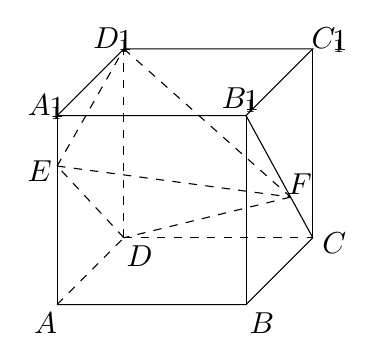
\begin{tikzpicture}[x=1bp,y=-1bp,
  every node/.style={inner sep=0,font=\fontsize{10.5pt}{12.6pt}\selectfont},
  line cap=butt, line join=miter]
  \draw[line width=0.398bp] (15.734,106.629) -- (83.746,106.629) -- (107.789,82.586);
  \draw[line width=0.398bp] (15.734,38.617) -- (83.746,38.617) -- (107.789,14.574) -- (39.777,14.574) -- (15.734,38.617);
  \draw[line width=0.398bp] (83.746,106.629) -- (83.746,38.617);
  \draw[line width=0.398bp] (107.785,82.586) -- (107.785,14.574);
  \draw[line width=0.398bp] (15.734,106.629) -- (15.734,38.617);
  \draw[line width=0.398bp] (83.746,38.617) -- (107.789,82.586);
  \draw[line width=0.398bp, dash pattern=on 2.989bp off 2.989bp] (15.734,106.629) -- (39.777,82.586);
  \draw[line width=0.398bp, dash pattern=on 2.989bp off 2.989bp] (39.777,82.586) -- (107.785,82.586);
  \draw[line width=0.398bp, dash pattern=on 2.989bp off 2.989bp] (39.777,82.586) -- (39.777,14.574);
  \draw[line width=0.398bp, dash pattern=on 2.989bp off 2.989bp] (39.777,82.586) -- (15.734,56.754);
  \draw[line width=0.398bp, dash pattern=on 2.989bp off 2.989bp] (15.734,56.754) -- (39.777,14.574);
  \draw[line width=0.398bp, dash pattern=on 2.989bp off 2.989bp] (39.777,14.574) -- (99.773,67.93);
  \draw[line width=0.398bp, dash pattern=on 2.989bp off 2.989bp] (99.773,67.93) -- (39.777,82.586);
  \draw[line width=0.398bp, dash pattern=on 2.989bp off 2.989bp] (15.734,56.754) -- (99.773,67.93);
  \node[anchor=base west] at (28.62,14.4) {$D_1$};
  \node[anchor=base west] at (37.31,15.29) {$1$};
  \node[anchor=base west] at (107.11,14.4) {$C_1$};
  \node[anchor=base west] at (114.62,15.29) {$1$};
  \node[anchor=base west] at (74.85,36.02) {$B_1$};
  \node[anchor=base west] at (82.82,36.91) {$1$};
  \node[anchor=base west] at (4.98,38.45) {$A_1$};
  \node[anchor=base west] at (12.85,39.35) {$1$};
  \node[anchor=base west] at (4.93,62.32) {$E$};
  \node[anchor=base west] at (98.72,67.05) {$F$};
  \node[anchor=base west] at (111.02,88.16) {$C$};
  \node[anchor=base west] at (40.57,93.09) {$D$};
  \node[anchor=base west] at (7.21,117.14) {$A$};
  \node[anchor=base west] at (84.8,117.14) {$B$};
\end{tikzpicture}
